% !TEX program = xelatex
% !BIB program = bibtex
% Connect6 Game Engine (tbe) — report, English version.
% Compile with XeLaTeX:  xelatex report_en && bibtex report_en && xelatex report_en && xelatex report_en
\documentclass[a4paper,10pt,twocolumn]{article}

\usepackage[margin=1.8cm,columnsep=0.7cm]{geometry}
\usepackage{fontspec}
\usepackage{polyglossia}
\setmainlanguage{english}
% Same font chain as the Russian draft: PT Serif (macOS, Overleaf) -> Times New Roman -> FreeSerif -> DejaVu Serif
\IfFontExistsTF{PT Serif}{\setmainfont{PT Serif}}{%
  \IfFontExistsTF{Times New Roman}{\setmainfont{Times New Roman}}{%
    \IfFontExistsTF{FreeSerif}{\setmainfont{FreeSerif}}{\setmainfont{DejaVu Serif}}}}
\IfFontExistsTF{PT Sans}{\setsansfont{PT Sans}}{\IfFontExistsTF{FreeSans}{\setsansfont{FreeSans}}{\setsansfont{DejaVu Sans}}}
\IfFontExistsTF{PT Mono}{\setmonofont[Scale=0.9]{PT Mono}}{\setmonofont[Scale=0.85]{DejaVu Sans Mono}}

\usepackage{amsmath,amssymb}
\usepackage{graphicx}
\usepackage{booktabs,tabularx,multirow}
\usepackage[table]{xcolor}
\usepackage{caption,subcaption}
\usepackage{enumitem}
\newenvironment{points}{\begin{enumerate}[label=(\arabic*),leftmargin=*,itemsep=2pt,topsep=3pt]}{\end{enumerate}}
\usepackage{tikz}
\usetikzlibrary{positioning,arrows.meta,calc,fit,backgrounds,shapes.misc}
\usepackage{pgfplots}
\pgfplotsset{compat=1.17}
\usepackage[round,authoryear]{natbib}
\setcitestyle{aysep={,},citesep={;}}
\usepackage{titlesec}
\usepackage[colorlinks=true,citecolor=blue!55!black,linkcolor=black,urlcolor=blue!55!black]{hyperref}
\usepackage{url}
\usepackage{stfloats}

\captionsetup{font=small,labelfont=bf,skip=4pt}
\titleformat*{\section}{\large\bfseries}
\titleformat*{\subsection}{\normalsize\bfseries}
\setlength{\parskip}{0.2em}
\newcommand{\todo}[1]{\textcolor{red}{[#1]}}
\newcommand{\code}[1]{\texttt{#1}}
\definecolor{cblue}{HTML}{2A78D6}
\definecolor{corange}{HTML}{EB6834}
\definecolor{cgreen}{HTML}{1BAF7A}
\definecolor{board}{HTML}{E2C27A}
\renewcommand{\arraystretch}{1.12}

% ---------- board drawing helpers (column c, row r; row A at the top, as in the GUI)
\tikzset{
  bstone/.style={circle,fill=black,inner sep=0pt,minimum size=3.4mm},
  wstone/.style={circle,fill=white,draw=black,line width=0.4pt,inner sep=0pt,minimum size=3.4mm},
  xmark/.style={cross out,draw=red,line width=1pt,inner sep=0pt,minimum size=2.4mm},
}
% \board{c0}{c1}{r0}{r1}: grid from column c0 to c1, rows r0 to r1, with letters
\newcommand{\board}[4]{%
  \fill[board] (#1-0.6,-#3+0.6) rectangle (#2+0.6,-#4-0.6);
  \foreach \c in {#1,...,#2} {\draw[black!60,line width=0.3pt] (\c,-#3) -- (\c,-#4);
     \node[font=\tiny\ttfamily,above] at (\c,-#3+0.45) {\pgfmathparse{int(\c+64)}\char\pgfmathresult};}
  \foreach \r in {#3,...,#4} {\draw[black!60,line width=0.3pt] (#1,-\r) -- (#2,-\r);
     \node[font=\tiny\ttfamily,left] at (#1-0.45,-\r) {\pgfmathparse{int(\r+64)}\char\pgfmathresult};}
}
\newcommand{\B}[2]{\node[bstone] at (#1,-#2) {};}
\newcommand{\W}[2]{\node[wstone] at (#1,-#2) {};}

\title{\textbf{Connect6 Game Engine}\\[0.3em]\large (engine: \texttt{tbe})}
\author{Tamara Besedina}
\date{November 2026}

\begin{document}
\maketitle
\begin{abstract}
\noindent
The goal of this work is a Connect6 engine that is compatible with the Connect6GUI/\allowbreak{}Connect6Engine interface \citep{connect6gui}, answers in real time, and uses evaluation-function weights, including weights learned with a machine-learning method \citep{statement}. The \code{tbe} engine was developed in five versions: v1 is a minimax search to a depth of two full moves; v2 adds alpha-beta pruning with move ordering and checks for immediate wins and defences; v3 adds an evaluation function with threats after Wu and Huang and connectivity after Liu; v4 adds quiescence search and forward pruning (forward pruning alone makes the search 2.7 times faster and compensates most of the cost of quiescence); v5 learns the weights by bootstrapping from search, which in the end showed that the original weights are better, so v5 is effectively the same as v4. Learning converges reproducibly from different starting points but does not make the engine stronger (45.8\,\% of the points against the hand-tuned weights). The final version passes all 12 test positions (win and defence in 1--3 moves) against Cloudict, survives 11 of its own moves on average against it from opening positions (v1: 6.5), and takes second place in the tournament after Cloudict.
\end{abstract}

% =====================================================================
\section{Introduction}

Connect6 is a two-player game of the $k$-in-a-row family. Black opens with a single stone; after that the players take turns placing \emph{two} stones on empty intersections of a $19\times19$ board. The first player to form a line of six or more stones horizontally, vertically or diagonally wins. The 1--2--2 rule makes the game balanced: after their own move, each player has exactly one stone more on the board than the opponent \citep{wu2005family}.

The game is very hard to search: on an empty board a move is chosen from $\binom{361}{2}\approx 65\,000$ pairs of cells, and in the middle game from tens of thousands. Even a depth of two full moves is therefore impossible without a strong restriction of candidates, pruning, and a good position evaluation.

The work is organised as a chain of versions from v1 to v5, adding improvement. v4 added two techniques at once (quiescence and forward pruning); their contributions were separated in a dedicated experiment (Section~\ref{sec:ablation}). All experiments were run locally on a MacBook Air with Apple M1, 8\,GB RAM, macOS 26.5.2: games against a human through the ConnectMore GUI, tests, the tournament and training from the terminal. An example is shown on Fig.~\ref{fig:v2game}. Code: \href{https://github.com/tomabes/connect6_engine_tbe}{GitHub link}.

\begin{figure}[h]
\centering
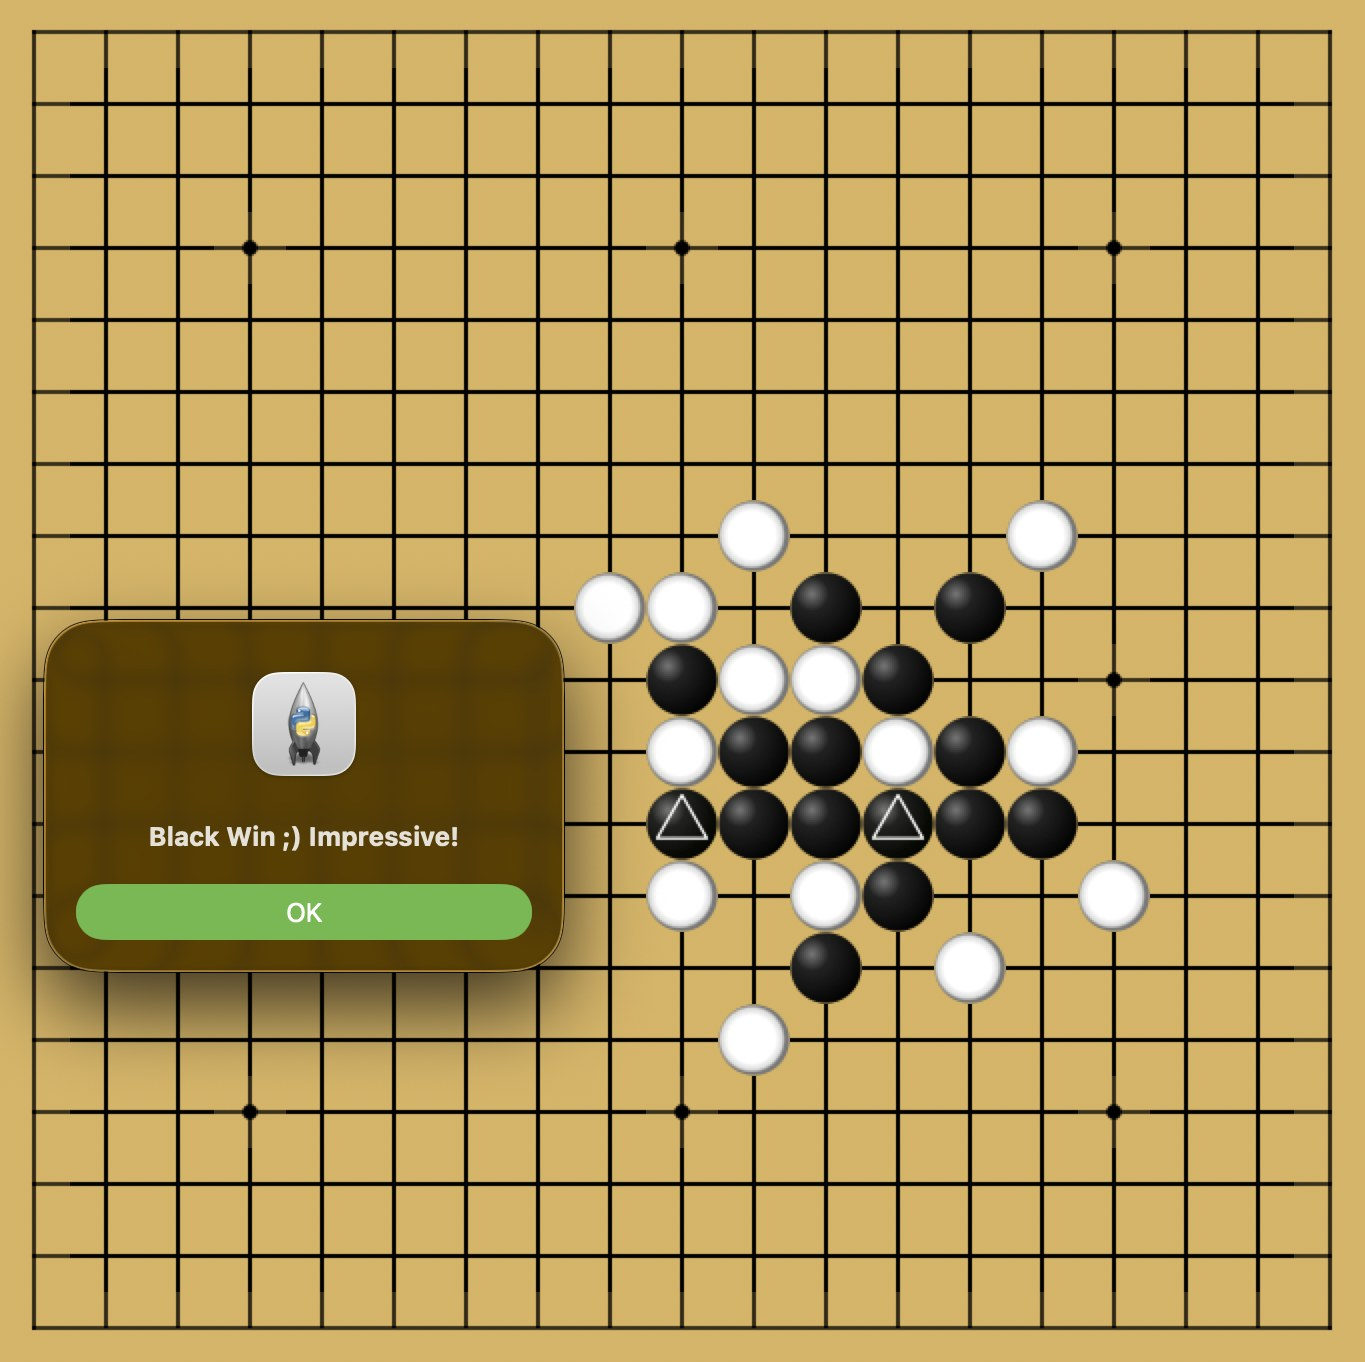
\includegraphics[width=0.48\textwidth]{figures/v2_vs_human.jpg}
\caption{v2 (Black) against a human in the GUI.}
\label{fig:v2game}
\end{figure}

\begin{figure*}[t]
\centering
\resizebox{\textwidth}{!}{%
\begin{tikzpicture}[
  box/.style={draw,rounded corners=2pt,align=center,font=\small,minimum height=9mm,inner sep=4pt,fill=white},
  ext/.style={box,fill=black!6},
  arr/.style={-{Stealth[length=2mm]},thick},
  lab/.style={font=\scriptsize,align=center}]
\node[ext] (gui) {ConnectMore GUI\\ / \code{benchmark.py}, \code{train.py}};
\node[box,right=1.6cm of gui] (main) {\code{main.py}\\ start-up};
\node[box,right=0.9cm of main] (ge) {\code{game\_engine.py}\\ protocol, game board,\\ time limit};
\node[box,right=1.5cm of ge] (se) {\code{search\_engine.py}\\ move generator $\cdot$ evaluation\\ alpha-beta $\cdot$ quiescence $\cdot$ FP};
\node[box,below=0.8cm of ge] (tools) {\code{tools.py}\\ moves, win check, printing};
\node[box,below=0.8cm of se] (def) {\code{defines.py}\\ constants, \code{EVAL\_WEIGHTS}};
\node[ext,right=0.9cm of def] (lw) {\code{learned\_weights.json}\\ (v5)};
\draw[arr] (gui.north east) to[bend left=12] node[lab,above] {stdin: \code{new}, \code{move},\\ \code{next}, \code{depth} \ldots} (ge.north west);
\draw[arr] (ge.south west) to[bend left=12] node[lab,below] {stdout: \code{move XXXX}\\ stderr: \code{metrics \{\ldots\}}} (gui.south east);
\draw[arr] (main) -- (ge);
\draw[arr] (ge) -- node[lab,above] {position,\\ budget} (se);
\draw[arr] (se) -- (tools);
\draw[arr] (ge) -- (tools);
\draw[arr] (def) -- (se);
\draw[arr] (lw) -- (def);
\end{tikzpicture}}
\caption{Architecture of the tbe engine and the flow of commands between the GUI, experiment scripts, and the engine. The modules are the same in all versions; mainly \code{search\_engine.py} changes from version to version.}
\label{fig:arch}
\end{figure*}

% =====================================================================
\section{State of the Art}\label{sec:sota}

\subsection{k-in-a-Row Games and Connect6}
Wu and Huang \citeyearpar{wu2005family} introduced the family of Connect($m,n,k,p,q$) games and proposed Connect6 = Connect(19,19,6,2,1) as a fair game. The key concept we take from their work is the \emph{threat}: a position in which the opponent has to spend a certain number of stones to avoid losing on the next move. If one stone is enough to defend, it is a single threat; if two are needed, a double threat; if two are not enough, the player with the threat wins. Since two stones are placed per move, a dead four (one end blocked) gives a single threat and an open four gives a double threat. The authors also stress that overlapping lines cannot be counted as independent threats and that the second stone of a move should be chosen after the first one has been placed.

\subsection{Game-Tree Search}
The basic algorithm is depth-limited minimax with a static evaluation at the leaves \citep{russell2020aima}. Alpha-beta gives the same result but prunes branches that cannot affect the decision; with perfect move ordering the number of nodes drops to roughly the square root of minimax \citep{knuth1975alphabeta}, so move ordering is an essential part of alpha-beta. A fixed depth causes the \emph{horizon effect}: a threat just beyond the search limit is not seen. Quiescence search continues the search at non-quiet leaves using tactical moves only \citep{russell2020aima}. Forward pruning discards in advance the moves that look weak according to a heuristic, trading accuracy for speed. The transposition tables, history heuristic and opening books suggested in the guide \citep{statement} were not implemented.

\subsection{Connect6-Specific Methods}
The strongest Connect6 programs rely on threat-space search, introduced by Allis for Gomoku \citep{allis1994}: only moves that create threats are considered, which makes it possible to find forced wins at a large depth. A special case is VCF (victory by continuous fours), a sequence of moves each of which creates a threat; this is how Cloudict finds its wins. Wu and Lin \citeyearpar{wu2010rzop} build on this idea a proof search over ``relevance zones'', the areas of the board where any defence must lie. Liu \citeyearpar{liu_defensive} complements threat search with a defensive strategy and an evaluation of potential lines: the influence of a stone decreases with distance and does not pass through an opponent's stone. We use this idea in the connectivity feature.

\subsection{Learning the Evaluation Function}
An evaluation is often written as a linear combination of features (lines, threats) with weights. In NCTU6, a multiple Computer Olympiad champion in Connect6, the weights were first tuned by hand from games against strong players and then refined with TD(0) learning, which gave 57.95\,\% wins against the original version \citep{wu2012td}. The course guide suggests a genetic algorithm \citep{statement}: a population of weight sets whose fitness is the result of games between them. The alternative is learning from positions: TD-Leaf \citep{baxter2000tdleaf} fits the evaluation to the search result from later positions, bootstrapping from game-tree search \citep{veness2009bootstrapping} fits it to the search value in the same position, and Texel tuning \citep{texel} minimises a logistic error between the evaluation and a label of the position.

A genetic algorithm was not implemented because fitness in a GA is the result of games: evaluating a single weight set needs dozens of games, and a generation needs hundreds. Bootstrapping gives a label for \emph{every} position rather than one per game, together with a differentiable error, so self-play give several thousand training examples and allow gradient-based optimisation.

\subsection{Reference Opponent Cloudict}
Cloudict \citep{cloudict} is an open-source Connect6 engine written in C++: alpha-beta to a given depth (2 in our setup) with VCF search. It serves as the reference opponent in all tests.

% =====================================================================
\section{Development}\label{sec:dev}

\subsection{Architecture}
All versions share the same five-module structure given by the teacher's template (Fig.~\ref{fig:arch}): \code{main.py} starts the engine, \code{game\_engine.py} parses the protocol commands, \code{search\_engine.py} contains the move generator, the evaluation and the search, \code{defines.py} holds constants and weights, and \code{tools.py} the board and the win check. The $19\times19$ board is stored in a $21\times21$ array with a border. Protocol answers go to stdout and search metrics (nodes, cut-offs, depth, time) to stderr: the GUI ignores them, while the experiment scripts read them.

\subsection{Communication Protocol and Time Control}
The engine supports all commands of the assignment (Table~\ref{tab:protocol}). As the assignment specifies, \code{depth N} sets a limit of $N$ seconds per move rather than a search depth. Time is controlled as follows: the search is iterative (depth 1 first, then 2), the timer is checked at every node, and when the budget runs out the engine returns the best move of the last \emph{fully} completed depth. A small part of the budget is kept for printing the answer.

\begin{table*}[t]
\centering
\caption{Commands of the Connect6GUI/\allowbreak{}Connect6Engine protocol.}
\label{tab:protocol}
\begin{tabularx}{\textwidth}{@{}lX@{}}
\toprule
Command & Action \\
\midrule
\code{name} & answers \code{name tbe} \\
\code{new black} / \code{new white} & new game; the engine plays the given colour \\
\code{new xxx}, \code{black XXXX}, \code{white XXXX} & reset and rebuild an arbitrary position move by move (letters A--S) \\
\code{next} & compute a move for the side to move \\
\code{move XXXX} & place the opponent's move and immediately answer with its own (\code{move JKJL}; a one-stone move is \code{move JJ}) \\
\code{depth N} & time limit of $N$ seconds per move (not the tree depth) \\
\code{print}, \code{help}, \code{exit}/\code{quit} & print the board, help, quit \\
\code{vcf}, \code{unvcf} & accepted and ignored, as the assignment requires \\
\bottomrule
\end{tabularx}
\end{table*}

\subsection{v1: Minimax Baseline}
The first version meets the requirements of the first session of the guide.
\emph{End of game}: after each move the engine checks whether the placed stone completed six in a row in one of the four directions; a full board without a winner is a draw.
\emph{Move generator}: candidates are the empty cells within a radius of 3 of any stone; they are ranked by a simple local score, the 12 best cells are kept, and up to 24 pairs are built from them (a pair is scored by the sum of its cell scores). This generator is deliberately narrow: searching all pairs is impossible even at depth one.
\emph{Evaluation}: for every six-cell window without opponent stones the engine counts its own stones; the evaluation is the black sum minus the white sum, a win is $\pm10^6$ and a draw is 0.
\emph{Search}: minimax to a depth of 2 full moves (a move and the reply).

\begin{table*}[b]
\centering
\caption{Features of the evaluation function and their hand-tuned weights used in v3, v4, and v5.}
\label{tab:features}
\begin{tabularx}{\textwidth}{@{}lrX@{}}
\toprule
Feature & Weight & Meaning \\
\midrule
\code{line\_1}\ldots\code{line\_5} & 1, 4, 16, 64, 256 & six-cell windows with 1\ldots5 own stones and no opponent stones; each stone multiplies the weight by 4 \\
\code{threat\_1} & 600 & all immediate wins can be blocked with one stone (dead four) \\
\code{threat\_2} & 3000 & two stones are needed (open four) \\
\code{threat\_3} & 15000 & two stones are not enough, so there is no defence \\
\code{connectivity} & 2 & sum of $(6-d)$ over pairs of own stones on one unblocked line, $d\le5$ \\
\bottomrule
\end{tabularx}
\end{table*}

\subsection{v2: Alpha-Beta Pruning and Move Ordering}
\emph{Alpha-beta.} The method is built directly on the v1 minimax with the same terminal conditions and depth limit; on the same tree it returns the same move (checked by a test) but prunes branches when $\alpha\ge\beta$.

\emph{Ordering and forced moves.} Alpha-beta is only efficient when strong moves are examined first \citep{knuth1975alphabeta}, so the generator became smarter. (1) If an immediate win exists, only winning pairs are proposed. (2) Otherwise, all opponent windows with 4--5 stones are collected and only pairs that block \emph{all} of the opponent's ways to win on the next move are proposed; these cells enter the candidate list regardless of the limit of 12. If no two-stone defence exists, the search continues with ordinary moves so that the loss is evaluated honestly. (3) In a quiet position a pair is scored by the joint change of all affected windows: the two stones of one move can strengthen the same line, which the sum of individual cell scores does not see.

\emph{Weighted evaluation.} The stone count in a window was replaced by a weight that grows by a factor of 4 per stone: 1, 4, 16, 64, 256 for a window with 1\ldots5 own stones (justified in Section~\ref{sec:v3}). Figure~\ref{fig:v2game} shows an example game of v2 against a human.

\subsection{v3: Threat-Based Evaluation}\label{sec:v3}
The third version implements our own evaluation function based on the literature. Nine features are computed for each colour (Table~\ref{tab:features}, Fig.~\ref{fig:features}):

\begin{itemize}\itemsep0pt
\item \code{line\_1}\ldots\code{line\_5}: the number of six-cell windows that contain 1\ldots5 stones of this colour and no opponent stones (windows that can still become a six);
\item \code{threat\_1}, \code{threat\_2}, \code{threat\_3}: the threat after Wu and Huang \citeyearpar{wu2005family}. For every window with 4--5 stones the engine stores the empty cells that would complete it, and then finds the minimum number of stones that block \emph{all} these sets (taking intersections between directions into account). The flag \code{threat\_1} means one stone is enough, \code{threat\_2} that two are needed, \code{threat\_3} that two are not enough;
\item \code{connectivity}, an idea from Liu \citeyearpar{liu_defensive}: along each line, split by opponent stones into segments at least six cells long, every pair of own stones at distance $d\le5$ contributes $6-d$. Close stones are worth more, and the influence does not pass through an opponent stone.
\end{itemize}

The position evaluation is a weighted difference of the features:
\begin{equation}
E=\sum_{i} w_i\,\bigl(f_i^{\text{black}}-f_i^{\text{white}}\bigr),
\label{eq:eval}
\end{equation}
where $E>0$ means Black is better; a win is $\pm10^6$ regardless of the weights.

\begin{figure*}[t]
\centering
\begin{subfigure}[t]{0.36\textwidth}\centering
\begin{tikzpicture}[scale=0.42]
\board{1}{12}{1}{3}
\B{4}{2}\B{5}{2}\B{7}{2}\W{11}{2}
\draw[cblue,line width=1.2pt,rounded corners=2pt] (1.55,-1.62) rectangle (7.45,-2.38);
\draw[cgreen,line width=1.2pt,rounded corners=2pt,dashed] (2.55,-1.5) rectangle (8.45,-2.5);
\draw[corange,line width=1.2pt,rounded corners=2pt] (5.55,-1.75) rectangle (11.45,-2.25);
\end{tikzpicture}
\caption{six-cell windows: the blue and green ones contain 3 black stones each (\code{line\_3}); the orange one contains a white stone and is not counted}
\end{subfigure}\hfill
\begin{subfigure}[t]{0.28\textwidth}\centering
\begin{tikzpicture}[scale=0.42]
\board{1}{9}{1}{3}
\W{2}{2}\B{3}{2}\B{4}{2}\B{5}{2}\B{6}{2}
\node[xmark] at (7,-2) {};
\end{tikzpicture}
\caption{dead four: all candidate windows are blocked by one stone ($\times$), which is \code{threat\_1}}
\end{subfigure}\hfill
\begin{subfigure}[t]{0.30\textwidth}\centering
\begin{tikzpicture}[scale=0.42]
\board{1}{10}{1}{3}
\B{4}{2}\B{5}{2}\B{6}{2}\B{7}{2}
\node[xmark] at (3,-2) {};\node[xmark] at (8,-2) {};
\end{tikzpicture}
\caption{open four: the windows are completed by the cell pairs, so the defence needs two stones, which is \code{threat\_2}}
\end{subfigure}
\caption{Evaluation features.}
\label{fig:features}
\end{figure*}

\emph{Justification of the hand-tuned weights.} The structure of the \code{line\_k} features is standard for $k$-in-a-row games: for Gomoku, Szőts and Harmati \citeyearpar{szots2018gomoku} count windows of length five without opponent stones and give a window with $n$ stones the weight $m^n$ (with $m=10$ tuned through play). We use the same rule for windows of length six but with base 4. The base is smaller because two stones are placed per move in Connect6: a line can rise by two levels in a single move, and with $m=10$ the evaluation would be determined by the single longest line, while shorter lines would no longer affect move choice. Learning in v5 indirectly supports this choice: the ratio \code{line\_2}/\code{line\_1} in the learned weights stayed close to 4 (Section~\ref{sec:learning-results}). A linear combination of lines and threats with hand-tuned weights is the same scheme NCTU6 used before its TD learning \citep{wu2012td}. The threat weights were chosen from constraints: each threat level is 5 times stronger than the previous one; a single threat (600) outweighs several \code{line\_4} fours because it forces the opponent to spend stones; and the upper bound of the whole feature sum stays far below the win score of $10^6$. Connectivity is a weak positional feature, so its weight (2) is comparable to \code{line\_1}--\code{line\_2}.

\begin{table*}[b]
\centering
\caption{Search metrics in GUI games against a human (terminal logs, 4\,s limit).}
\label{tab:gui}
\begin{tabular}{@{}lrrrrrr@{}}
\toprule
Version & moves & nodes & pruned & time, s (max) & depth & time-outs \\
\midrule
v1 & 10 & 622 & 0 & 0.30 (0.33) & 2.0 & 0 \\
v2 & 6 & 97 & 246 & 0.13 (0.18) & 2.0 & 0 \\
v3 & 5 & 102 & 439 & 1.06 (1.48) & 2.0 & 0 \\
v4, QS = 2 (before tuning) & 5 & 356 & 1797 & 3.37 (3.98) & 1.2 & 4/5 \\
v4, QS = 1 (final) & 5 & 189 & 360 & 1.12 (3.24) & 2.0 & 0 \\
\bottomrule
\end{tabular}
\end{table*}

\emph{Pair generator of v3.} The v2 checks are kept. In a quiet position, following Wu and Huang, the first stone of a pair is temporarily placed on the board, and the candidates for the second stone are scored in the modified position. Pairs are sorted by outcome, then by threat strength (0/1/2/$\ge3$), by the number of live fours and fives, and by the evaluation~(\ref{eq:eval}); up to 24 pairs go into the search. The depth remained 2 full moves, but the evaluation became much more expensive (Section~\ref{sec:speed}).

\subsection{v4: Quiescence Search and Forward Pruning}\label{sec:v4}
At depth 2 the horizon effect is especially dangerous: an opponent win on the third move is not seen. v4 therefore adds two techniques from the fourth session of the guide; both can be switched off with the flags \code{--no-quiescence} and \code{--no-forward-pruning}, which later made it possible to measure them separately.

\emph{Quiescence search.} At the depth limit, instead of the static evaluation, the engine runs a short tactical continuation: its own immediate wins first, otherwise the forced defences against an opponent win. In a quiet position the v3 evaluation is returned immediately and ordinary pairs are not generated. Under a threat the engine cannot ``stand pat'': if no pair blocks all of the opponent's wins, a losing score is returned. The extension depth is limited by \code{Q\_MAX\_DEPTH} and by the global timer.

\emph{Forward pruning.} Ordinary pairs are first scored by the cheap change of the affected windows (the v2 score), and only the best 24 (\code{FP\_PRESELECT}) go through the expensive v3 threat and connectivity analysis; after full ranking at most 8 quiet pairs remain (\code{FP\_MAX\_QUIET\_MOVES}). Forcing pairs are never cut by this limit, and when either side has an immediate threat pruning is switched off completely and the v3 generator is used.

\begin{figure*}[t]
\centering
\begin{subfigure}[t]{0.32\textwidth}\centering
\begin{tikzpicture}[scale=0.3]
\board{3}{17}{3}{17}
\B{6}{10}\B{7}{10}\B{8}{10}\B{9}{10}
\W{8}{12}\W{12}{8}\W{5}{14}
\end{tikzpicture}
\caption{win1: an open four, six on the next move}
\end{subfigure}\hfill
\begin{subfigure}[t]{0.32\textwidth}\centering
\begin{tikzpicture}[scale=0.3]
\board{3}{17}{3}{17}
\B{7}{6}\B{8}{6}\B{9}{6}\B{14}{11}\B{14}{12}\B{14}{13}
\W{10}{10}\W{4}{14}\W{11}{15}
\end{tikzpicture}
\caption{win2: two open threes become two open fours, then six}
\end{subfigure}\hfill
\begin{subfigure}[t]{0.32\textwidth}\centering
\begin{tikzpicture}[scale=0.3]
\board{3}{17}{3}{17}
\B{5}{4}\B{6}{4}\B{7}{4}\B{11}{13}\B{12}{13}\B{10}{14}\B{10}{15}
\W{15}{7}\W{4}{9}\W{16}{16}
\end{tikzpicture}
\caption{win3: an open three and two twos crossing at J\,M}
\end{subfigure}
\caption{Test position patterns (the attacker is Black; a fragment of the board is shown, filler stones on the edges are omitted). In the defend$k$ categories the engine plays White in the same positions; for White the patterns are rotated by $90^\circ$.}
\label{fig:positions}
\end{figure*}

\emph{Tuning the quiescence depth.} Initially two tactical moves were allowed (\code{Q\_MAX\_DEPTH = 2}). In a game against a human through the GUI (4\,s limit) this caused a time-out in 4 of the 5 non-trivial moves: the search only completed depth 1 (Table~\ref{tab:gui}, row ``v4, QS = 2''). The problem was reproduced on two opening positions; with \code{Q\_MAX\_DEPTH = 1} depth 2 completed, and the chosen moves on four control positions were unchanged. After tuning there were no time-outs in a similar game, and the average time per move dropped from 3.37 to 1.12\,s.

The logs also confirm the cost of the v3 evaluation: on the first two moves v2 and v3 built the same tree (118 nodes, 506 pruned moves), but v3 spent 1.48\,s against 0.18\,s for v2, 8 times more, entirely because of the threat and connectivity features.

\begin{figure*}[b]
\centering
\begin{subfigure}[b]{0.49\textwidth}\centering
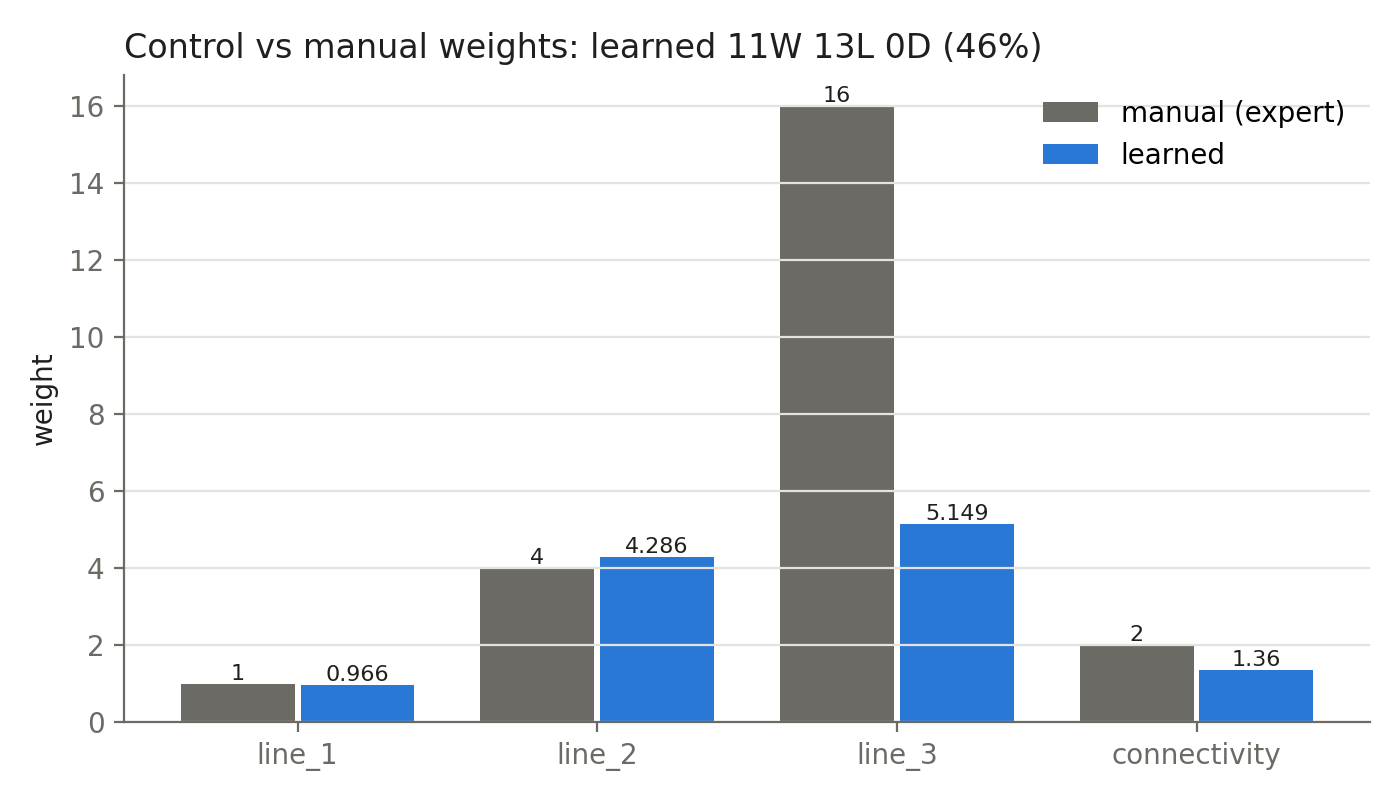
\includegraphics[width=\linewidth]{figures/weights_bar_manual.png}
\caption{hand-tuned and learned weights}
\end{subfigure}\hfill
\begin{subfigure}[b]{0.49\textwidth}\centering
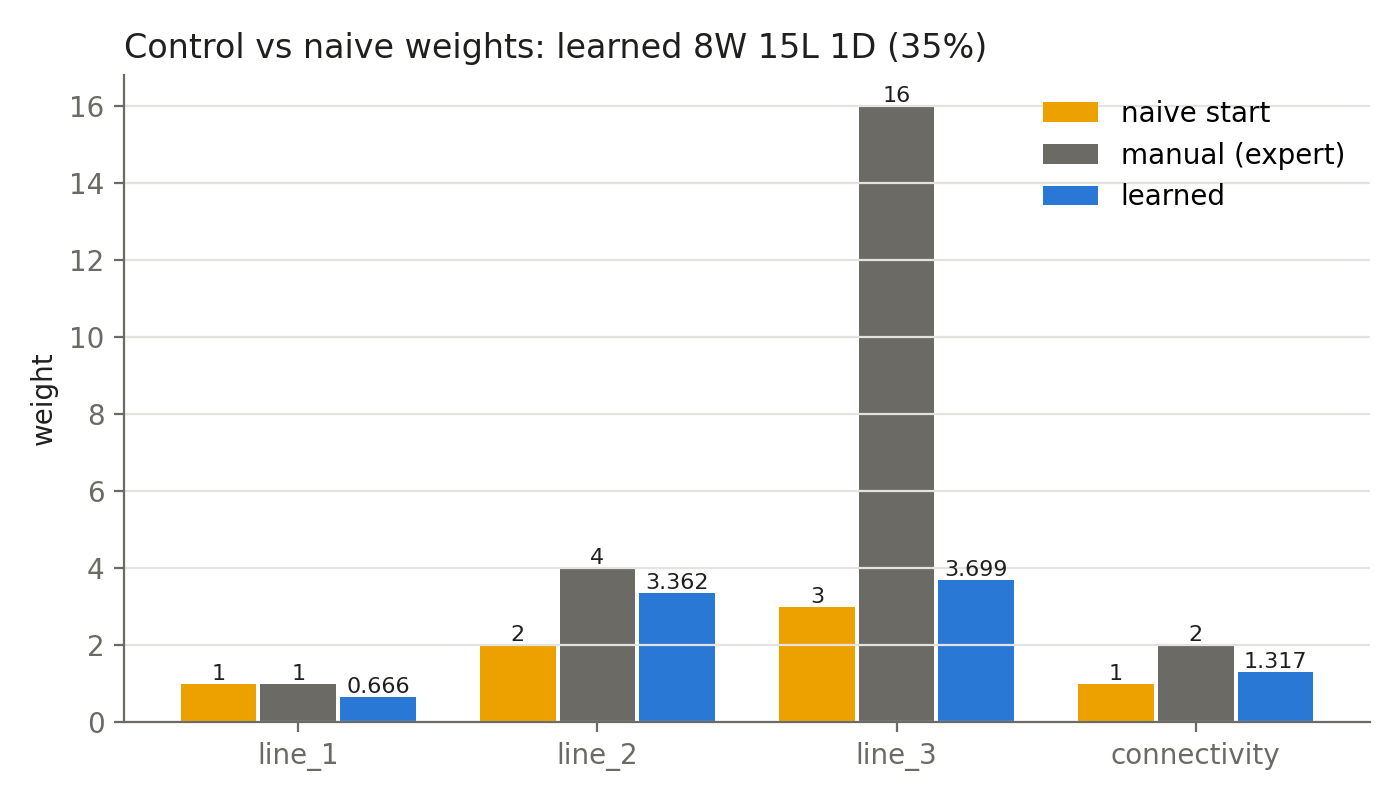
\includegraphics[width=\linewidth]{figures/weights_bar_naive.png}
\caption{naive, hand-tuned and learned weights}
\end{subfigure}
\caption{Final weights and the results of the control games (in the plot titles).}
\label{fig:weights}
\end{figure*}

\subsection{v5: Learning the Evaluation Weights}\label{sec:v5}
The fifth version uses the v4 search unchanged and adds weight learning (\code{train.py}). The learned weights are accepted only if they beat the hand-tuned ones both in error and in play.

\emph{Method is bootstrapping from search} \citep{veness2009bootstrapping,texel}. The static evaluation~(\ref{eq:eval}) learns to predict the value of a deeper search (the ``teacher'') in the same position. The teacher is a one-full-move search plus quiescence with the hand-tuned weights.

\emph{Data.} Self-play with 6 processes, from random openings near the centre; during the first 6 moves, with probability $\varepsilon=0.3$, the engine plays another of its four best moves instead of the best one, to diversify positions. Only \emph{quiet} positions, where no side has 4--5 stones in a window, are labelled. These are exactly the leaves where the engine applies the static evaluation, while tactics are handled by the move generator and quiescence. Moreover, in tactical positions the teacher's value is close to $\pm10^6$ and would dominate the error over all other positions. One run produced about 560 games and about 3\,600 positions; 20\,\% of the \emph{games} (not positions) were held out for validation, so that neighbouring positions of one game do not end up in both sets.

\emph{Error.} Both evaluations are mapped to a ``probability that Black wins'' with the sigmoid $\sigma(E/K)$, where the scale $K=108$ is the median of $|E_{\text{teacher}}|$; the error is the logistic loss (cross-entropy), as in Texel tuning \citep{texel}. The optimiser is Adam, with L2 regularisation towards the starting weights and early stopping on the validation error (Table~\ref{tab:hyper}).

\emph{Weights learned} are \code{line\_1}, \code{line\_2}, \code{line\_3} and \code{connectivity}. In quiet positions \code{line\_4}, \code{line\_5} and the threats are zero, there is no data for them, and they keep their hand-tuned values. The weights are bounded between 0.25 and 3.5--4 times the hand-tuned values and kept monotone, $\code{line\_1}<\code{line\_2}<\code{line\_3}<\code{line\_4}$. During training a side-to-move (tempo) term is added: the same position is better for the side that is to move. It is not needed in play: at a fixed depth the same side is to move in all leaves, so the term shifts all evaluations equally and does not change the choice of move.

\emph{Control and selection.} The learned weights play against the starting weights: 12 new openings $\times$ 2 colours, 3\,s per move, with a 40-move limit counted as a draw. The weights are accepted if the validation error is lower \emph{and} they score more than 50\,\% in the control games; otherwise the starting weights are kept.

To check that the procedure finds reasonable weights on its own rather than just staying near the hand-tuned ones, a second experiment was run, starting from ``naive'' weights \code{line\_1..3} = 1, 2, 3 (weight = number of stones) and \code{connectivity} = 1, with regularisation towards this naive start (not towards the hand-tuned weights, so as not to hint at the answer). The results are in Section~\ref{sec:learning-results}.

% =====================================================================
\section{Experimentation}\label{sec:exp}

\subsection{Methodology}
Experiments were run with the \code{benchmark.py} script. The opponent is Cloudict at depth 2 with VCF. Our engine's limit in the tests and the tournament is 3\,s per move. \emph{Test positions} were built following the fifth session of the guide (Fig.~\ref{fig:positions}). For three patterns (a win in 1, 2 and 3 moves) the engine plays the attacker (categories win1--3), and in the same position with the roles reversed it plays the defender (defend1--3). Each pattern is used twice: for Black, and rotated by $90^\circ$ for White. The stones needed to make the position legal are placed on the edge of the board, far from the pattern. A win$k$ test is passed if the engine wins within $k$ of its own moves; a defend$k$ test if it does not lose within 4 of its own moves. The start category is an ordinary opening (as White after \code{JJ}, as Black after \code{JJ IKKK}): we count how many of its own moves (up to 15) the engine survives against Cloudict. Search metrics are taken from the \emph{first} move, so all versions are compared on the same 14 positions.

\begin{figure*}[t]
\centering
\pgfplotsset{
  myax/.style={width=0.27\textwidth,height=4.2cm,ybar,ymin=0,axis lines*=left,
    ymajorgrids,grid style={black!12},tick label style={font=\scriptsize},
    label style={font=\scriptsize},title style={font=\small,align=center},
    legend style={font=\scriptsize,draw=none,fill=none},enlarge x limits=0.18,
    nodes near coords style={font=\tiny}}}
\begin{tikzpicture}
\begin{axis}[myax,bar width=6pt,symbolic x coords={v1,v2,v3,v4/v5},xtick=data,
   title={(a) search size},legend pos=north east,legend columns=1]
\addplot[fill=cblue,draw=none] coordinates {(v1,614) (v2,80) (v3,77) (v4/v5,126)};
\addplot[fill=corange,draw=none] coordinates {(v1,0) (v2,254) (v3,287) (v4/v5,363)};
\legend{nodes,pruned}
\end{axis}
\end{tikzpicture}\hfill
\begin{tikzpicture}
\begin{axis}[myax,bar width=10pt,symbolic x coords={v1,v2,v3,v4/v5},xtick=data,
   title={(b) first-move time, s},nodes near coords,nodes near coords align={vertical}]
\addplot[fill=cgreen,draw=none] coordinates {(v1,0.41) (v2,0.16) (v3,1.30) (v4/v5,1.43)};
\end{axis}
\end{tikzpicture}\hfill
\begin{tikzpicture}
\begin{axis}[myax,bar width=6pt,symbolic x coords={base,QS,FP,QS+FP},xtick=data,
   title={(c) v4, QS and FP: search size}]
\addplot[fill=cblue,draw=none] coordinates {(base,77) (QS,144) (FP,51) (QS+FP,137)};
\addplot[fill=corange,draw=none] coordinates {(base,287) (QS,451) (FP,98) (QS+FP,417)};
\end{axis}
\end{tikzpicture}\hfill
\begin{tikzpicture}
\begin{axis}[myax,bar width=10pt,symbolic x coords={base,QS,FP,QS+FP},xtick=data,
   title={(d) v4, QS and FP: time, s},nodes near coords,nodes near coords align={vertical}]
\addplot[fill=cgreen,draw=none] coordinates {(base,1.18) (QS,1.69) (FP,0.43) (QS+FP,1.37)};
\end{axis}
\end{tikzpicture}
\caption{Engine metrics: (a, b) by version; (c, d) v4 with quiescence (QS) and forward pruning (FP) switched off and on. Blue bars are expanded nodes, orange bars are pruned moves.}
\label{fig:metrics}
\end{figure*}

\subsection{Test Positions against Cloudict}
The results are in Table~\ref{tab:battery}.
\begin{points}
\item v1 fails win2, win3 and defend1: it has no explicit check for wins and defences, and its narrow generator (12 cells chosen by a simple score) does not always contain the required cells. From v2 on, all 12 tests are passed, thanks to the forced-move generator.
\item All versions, including v1, pass defend2 and defend3: Cloudict does not manage to convert these threats within 4 moves even against a weak defender, so these categories hardly separate the versions.
\item From the opening positions v2--v5 survive 11--12.5 of their own moves against Cloudict, while v1 survives only 6.5. The difference between v2, v3 and v4 (1--1.5 moves with two games per version) is within noise.
\end{points}

\begin{table}[h]
\centering
\small
\setlength{\tabcolsep}{2pt}
\caption{Test positions against Cloudict: passed / played.}
\label{tab:battery}
\begin{tabular}{@{}lcccccc|c@{}}
\toprule
Version & win1 & win2 & win3 & defend1 & defend2 & defend3 & start \\
\midrule
v1 & 2/2 & \cellcolor{red!12}0/2 & \cellcolor{red!12}0/2 & \cellcolor{red!12}0/2 & 2/2 & 2/2 & 6.5 \\
v2 & 2/2 & 2/2 & 2/2 & 2/2 & 2/2 & 2/2 & 11.5 \\
v3 & 2/2 & 2/2 & 2/2 & 2/2 & 2/2 & 2/2 & 12.5 \\
v4/v5 & 2/2 & 2/2 & 2/2 & 2/2 & 2/2 & 2/2 & 11.0 \\
\bottomrule
\end{tabular}
\end{table}

A caveat: in the win3 positions the defender's filler stones sometimes lie on a line with its other stones, which gives the defender counter-play. This makes the test slightly harder than intended (this is how v1 lost win3), but it does not change the outcome for v2--v5.

\begin{table*}[t]
\centering
\caption{v4 with QS and FP switched off and on, on the 14 test positions (3\,s per move). Metrics are first-move averages; q-nodes are quiescence calls; FP-pruned are pairs removed by forward pruning.}
\label{tab:ablation}
\begin{tabular}{@{}lccrrrrrrc@{}}
\toprule
Mode & tests & start & time, s & nodes & pruned & depth & q-nodes & FP-pruned & time-outs \\
\midrule
no QS, no FP & 12/12 & 12.5 & 1.18 & 77 & 287 & 2.00 & 0 & 0 & 0/14 \\
QS only & 12/12 & 10.5 & 1.69 & 144 & 451 & 1.64 & 131 & 0 & 5/14 \\
FP only & 12/12 & 13.5 & \textbf{0.43} & 51 & 98 & 2.00 & 0 & 159 & 0/14 \\
QS + FP (v4) & 12/12 & 11.0 & 1.37 & 137 & 417 & 1.71 & 127 & 137 & 4/14 \\
\bottomrule
\end{tabular}
\end{table*}

\begin{figure*}[b]
\centering
\begin{subfigure}[b]{0.328\textwidth}\centering
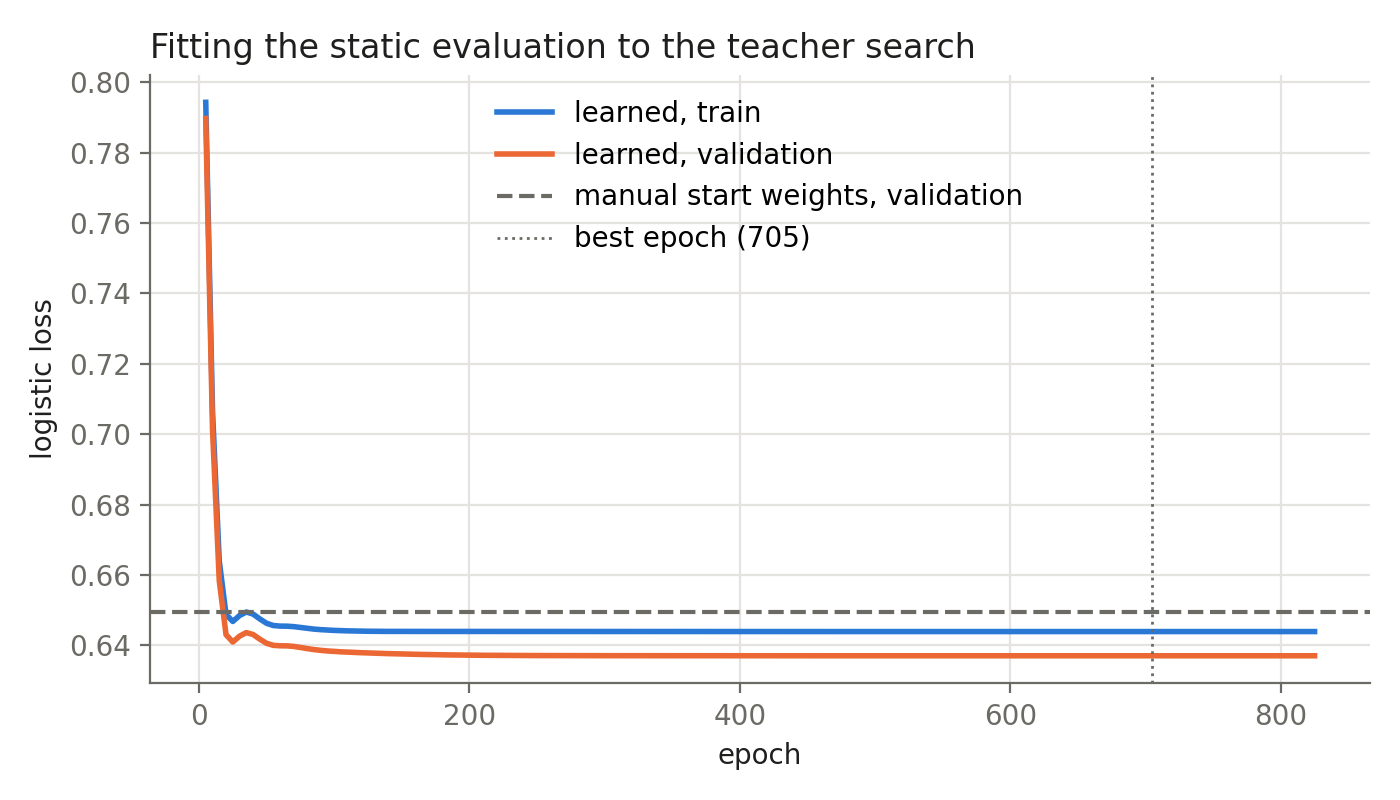
\includegraphics[width=\linewidth]{figures/loss_manual.png}
\caption{loss, start from hand-tuned weights}
\end{subfigure}\hfill
\begin{subfigure}[b]{0.328\textwidth}\centering
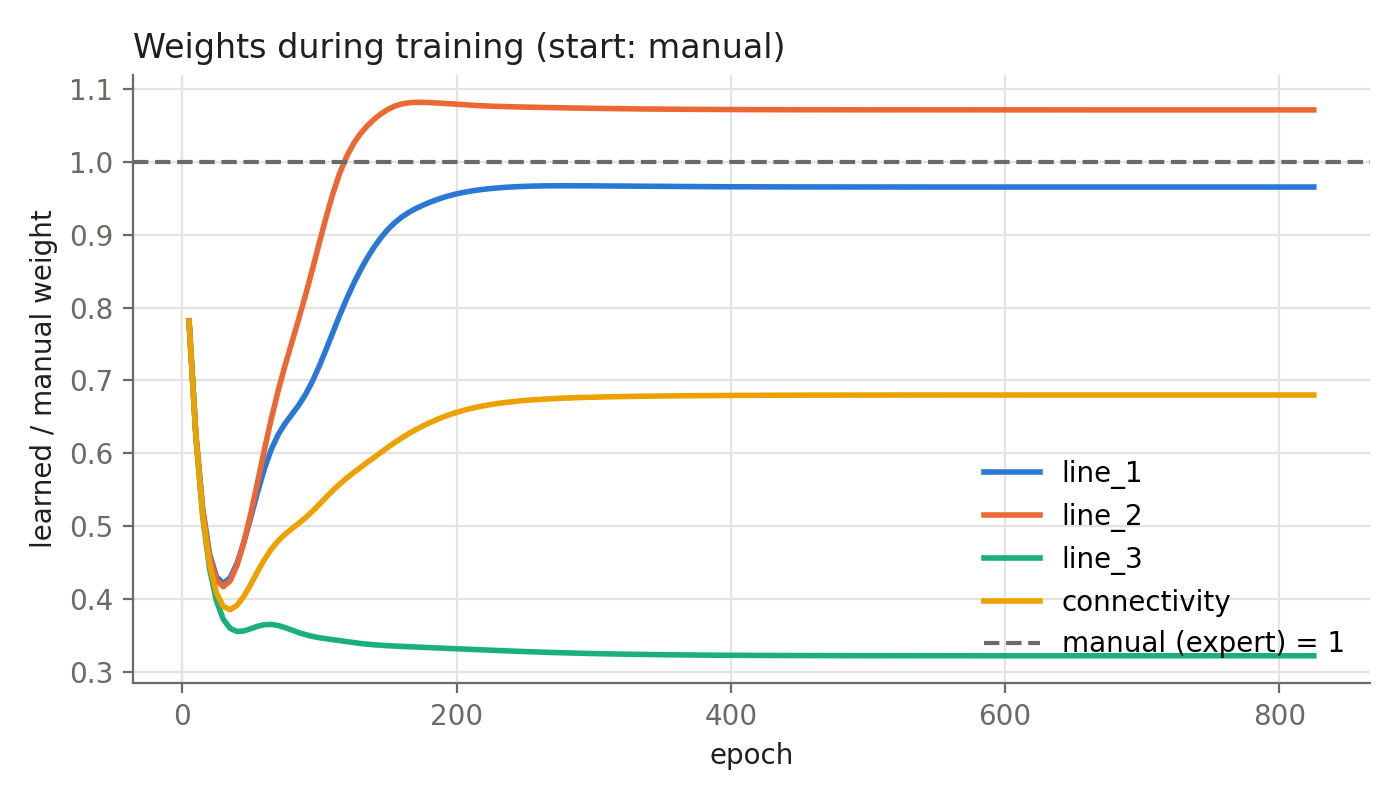
\includegraphics[width=\linewidth]{figures/weights_manual.png}
\caption{weights, start from hand-tuned}
\end{subfigure}\hfill
\begin{subfigure}[b]{0.328\textwidth}\centering
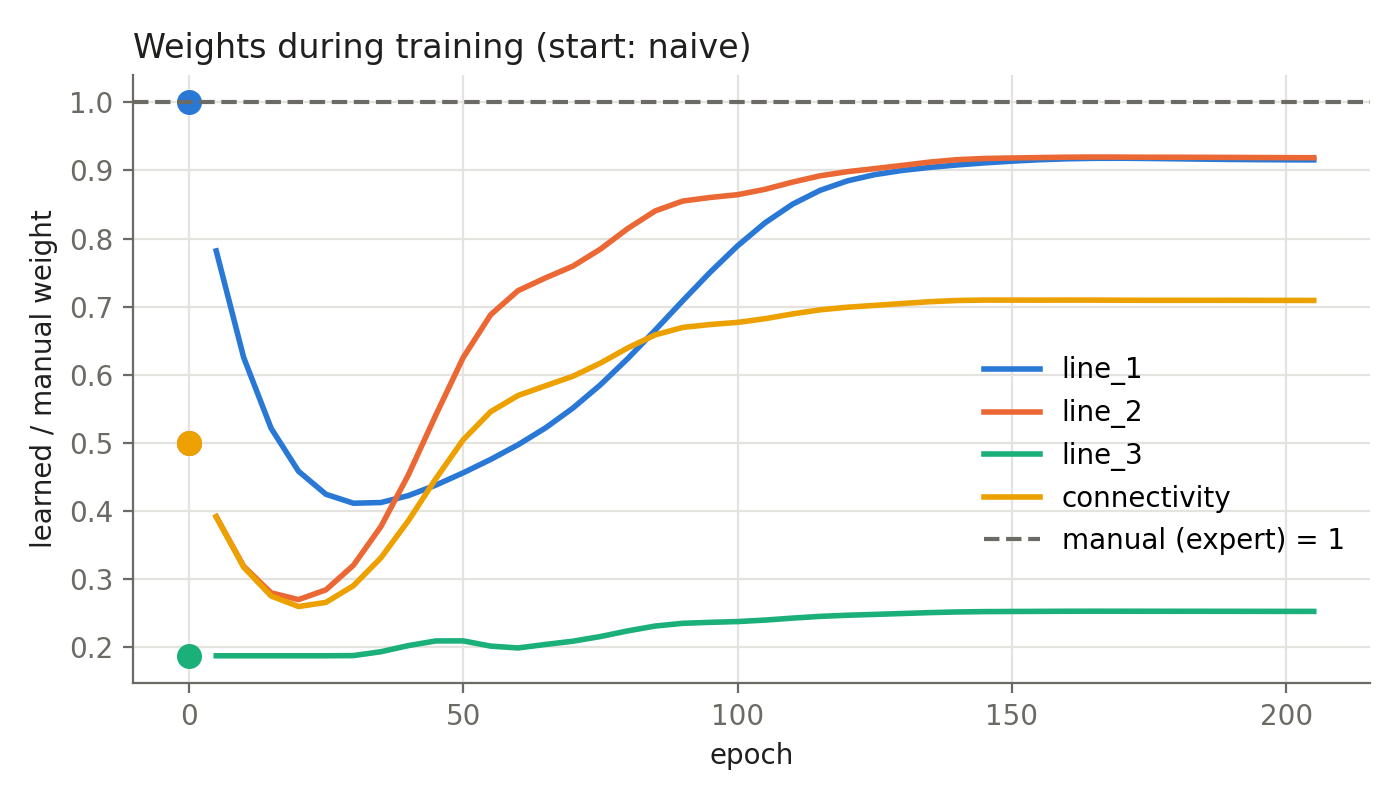
\includegraphics[width=\linewidth]{figures/weights_naive.png}
\caption{weights, start from naive (dots)}
\end{subfigure}
\caption{Training progress. (a) Logistic loss on train and validation when starting from the hand-tuned weights; the dashed line is the validation loss of the hand-tuned weights (0.6496), the best epoch is 705 (0.6371). (b, c) Weights as fractions of the hand-tuned values. The final weights are taken at the best epoch (705 and 85); the curves continue until early stopping. From both starts \code{line\_3} ends up in the range 3.7--5.2, coming from above (from 16) and from below (from 3).}
\label{fig:loss}
\end{figure*}

\subsection{Speed, Search Size and Memory}\label{sec:speed}
First-move metrics on the same 14 positions are given in Table~\ref{tab:metrics} and Fig.~\ref{fig:metrics}(a,\,b).
\begin{points}
\item Going from v1 to v2 (alpha-beta and move ordering) reduces the number of nodes by a factor of 7.7, from 614 to 80, and the time by a factor of 2.5 at the same depth of 2.
\item In v3 the number of nodes barely changes, but the time grows 8-fold, from 0.16 to 1.30\,s: the threat and connectivity analysis at every node is expensive.
\item In v4/v5 there are more nodes because of quiescence, and the average depth drops to 1.71: in some of the defend2 and defend3 positions the search hits the 3\,s limit and only completes depth 1. In normal play through the GUI the limit is 4\,s, and after tuning quiescence there were no time-outs (Table~\ref{tab:gui}).
\end{points}

\begin{table}[h]
\centering
\small
\setlength{\tabcolsep}{3pt}
\caption{First-move depth and memory averaged among 14 test positions.}
\label{tab:metrics}
\begin{tabular}{@{}lrrrrr@{}}
\toprule
Ver-n & depth & memory, MiB \\
\midrule
v1 & 2.00 & 17.6 \\
v2 & 2.00 & 18.0 \\
v3 & 2.00 & 18.6 \\
v4/v5 & 1.71 & 20.1 \\
\bottomrule
\end{tabular}
\end{table}

\emph{Memory.} The peak resident size of the process (\code{/usr/bin/time -l}, two moves with a 3\,s limit) is given in the last column of Table~\ref{tab:metrics}. All versions stay within 18--20\,MiB, most of which is taken by the Python interpreter itself; the new techniques add about 2.5\,MiB in total. Memory use is small by design: there are no transposition tables or caches, the recursion is at most three moves deep, and temporary stones are placed on and removed from a single board instead of copying it, so memory use is $O(\text{board}+\text{depth}\times\text{candidates})$ and does not grow with the number of nodes.

\subsection{v4: Quiescence vs Forward Pruning}\label{sec:ablation}
Both techniques were added to v4 at the same time, so their contributions were measured separately: the same set of 14 test positions was run for v4 in four modes, namely without either technique, with QS only, with FP only, and with both (the normal v4). The results are in Table~\ref{tab:ablation} and Fig.~\ref{fig:metrics}(c,\,d).
\begin{points}
\item This run is consistent with the main one: the mode without either technique gives exactly the same 77 nodes and 287 pruned moves as v3, and the QS+FP mode is close to the main v4 run (126 nodes, 1.43\,s, depth 1.71). The small difference comes from the time limit: the moment when the search is interrupted varies slightly from run to run.
\item Forward pruning is the more useful of the two techniques. It reduces the first-move time by a factor of 2.7, from 1.18 to 0.43\,s, and the number of nodes by a third, without a single time-out or a single failed test.
\item Quiescence, on the contrary, adds about 130 nodes and increases the time by a factor of 1.4. In 5 of the 14 positions the 3\,s limit is not enough and the search only completes depth 1. When forward pruning is enabled as well, part of this cost is recovered: the time drops from 1.69 to 1.37\,s, with 4 time-outs instead of 5.
\item The test results do not separate the modes: all four pass 12 out of 12. Immediate wins and defences are already found by the move generator (since v2), so extending the search by one tactical move with quiescence adds nothing here. The start values (from 10.5 to 13.5 moves) come from two games per mode, and the difference of 1--3 moves is not significant.
\end{points}
In summary, forward pruning is the only one of the two techniques that speeds the search up; in v4 it compensates most of the cost of quiescence, so v4 is about as fast as v3 (1.37--1.43\,s against 1.30\,s). The benefit of quiescence is not visible on our tests, while its cost under a 3\,s limit is noticeable. The final QS+FP configuration was not changed, and it is the one that played in the tournament.

\subsection{Weight Learning}\label{sec:learning-results}
The results of the two training runs, from the hand-tuned and from the naive weights, are given in Table~\ref{tab:learning}; training progress and the final weights are shown in Figs.~\ref{fig:loss} and~\ref{fig:weights}.
\begin{points}
\item The procedure works and reaches the same region of weights from different starting points. From the hand-tuned weights \code{line\_3} falls from 16 to 5.1, and from the naive weights it rises from 3 to 3.7; from the naive start \code{line\_2} rises from 2 to 3.4, almost matching the hand-tuned value of 4. The ratio \code{line\_2}/\code{line\_1} stays close to 4 in both runs, which supports the chosen base of 4.
\item At the same time, the loss function hardly distinguishes between weight sets: the hand-tuned and the naive weights give practically the same validation loss (0.650 and 0.648), and training improves it by only 1--2\,\%.
\item A lower loss does not translate into stronger play. In the control games the learned weights scored below 50\,\% in both runs: 45.8\,\% against the hand-tuned weights and 35.4\,\% against the naive ones. The learned weights undervalue \code{line\_3}, while threes matter in play: a three of the side to move becomes a five in a single move.
\item The cause most likely lies in the design of the features. Each feature is a difference ``black minus white'' and does not tell whose three it is: a three of the side to move is almost a win, a three of the opponent is not. The linear model averages these cases and undervalues \code{line\_3}. The tempo term does not fix this, since it is the same for all positions and does not depend on the features.
\item In the run from the hand-tuned weights the automatic selection rejected the learned weights, which is the right decision: v5 plays with the hand-tuned weights and is identical to v4. In the naive run the selection kept the naive starting weights; this run does not affect the weights the engine actually uses.
\end{points}

\subsection{Tournament}
All versions and Cloudict played a round robin: 2 openings (\code{JJ KJKK} and \code{JJ HHLL}) $\times$ 2 colours, 3\,s per move, a 30-move limit, 60 games in total. 16 games did not finish within 30 moves and were scored as draws (0.5 points each). The standings and head-to-head results are in Table~\ref{tab:tournament}.
\begin{table}[t]
\centering
\caption{Tournament standings (a win scores 1, a draw or an unfinished game 0.5). v4 and v5 played as separate entrants with identical results.}
\label{tab:tournament}
\begin{tabular}{@{}lrrrrr@{}}
\toprule
Player & points & W & L & D & games \\
\midrule
Cloudict & 19.0 & 18 & 0 & 2 & 20 \\
v4 & 11.0 & 8 & 6 & 6 & 20 \\
v5 & 11.0 & 8 & 6 & 6 & 20 \\
v3 & 9.0 & 5 & 7 & 8 & 20 \\
v2 & 8.5 & 5 & 8 & 7 & 20 \\
v1 & 1.5 & 0 & 17 & 3 & 20 \\
\bottomrule
\end{tabular}
\end{table}

\begin{points}
\item The ranking follows the order of the improvements: v1, then v2, v3, v4 = v5, and Cloudict.
\item v3 lost its head-to-head match against v2, 1.5:2.5: the new evaluation did not add strength by itself but slowed the search down 8-fold. v4 did not lose a single game either to v2 (2 wins, 2 draws) or to v3 (1 win, 3 draws). Given Section~\ref{sec:ablation}, a reasonable explanation is the speed-up from forward pruning, which lets the expensive v3 evaluation fit into the time limit.
\item All versions lose to Cloudict, but v2--v5 survive noticeably longer than v1 (11--12.5 own moves in the start tests against 6.5), and v2 and v3 each reached the 30-move limit once. Cloudict is stronger thanks to the speed of C++ and its VCF search many moves ahead, while our search covers two full moves.
\end{points}

\begin{table}[t]
\centering
\caption{Tournament head-to-head results: points of the row player against the column player (out of 4 games).}
\label{tab:h2h}
\begin{tabular}{@{}lccccc@{}}
\toprule
& v1 & v2 & v3 & v4/v5 & Cloudict \\
\midrule
v1 & --- & 0.5 & 0.0 & 0.5 & 0.0 \\
v2 & 3.5 & --- & 2.5 & 1.0 & 0.5 \\
v3 & 4.0 & 1.5 & --- & 1.5 & 0.5 \\
v4/v5 & 3.5 & 3.0 & 2.5 & 2.0$^{*}$ & 0.0 \\
Cloudict & 4.0 & 3.5 & 3.5 & 4.0 & --- \\
\bottomrule
\end{tabular}\\[2pt]
{\footnotesize $^{*}$ v4 against v5: 2:2, the games mirror each other (same engine).}
\end{table}

% =====================================================================
\section{Conclusions}\label{sec:concl}

We developed the Connect6 engine \code{tbe}, fully compatible with the course protocol, in five versions, and measured the contribution of each step.
\begin{points}
\item v1 (minimax, depth 2) became a working baseline: 614 nodes per move, failed tests win2, win3 and defend1, 6.5 moves against Cloudict.
\item v2 (alpha-beta, move ordering, forced moves) gave the largest gain: 7.7 times fewer nodes, all 12 tests passed, 11.5 moves against Cloudict.
\item v3 (threats after Wu and Huang, connectivity after Liu) made the evaluation more meaningful but 8 times more expensive; in the tournament it lost to v2 by 1.5:2.5.
\item v4 (quiescence, forward pruning) is the best version: second place in the tournament (11 points out of 20) with no losses to v2 or v3. A separate experiment showed that the speed-up comes from forward pruning (a factor of 2.7), while quiescence under a 3\,s limit mostly adds cost.
\item v5 (weight learning): the procedure converges reproducibly from different starting points but does not improve play (45.8\,\% of the points against the original weights), so the automatic selection kept the hand-tuned weights.
\end{points}

\emph{Main lessons.} The move generator and move ordering matter more than a sophisticated evaluation: almost all of the tactical strength appeared already in v2. An expensive evaluation only pays off when the search has time to apply it, which in our case is made possible by forward pruning. The learning procedure works, but it is limited by the features: they do not take into account whose turn it is, so the loss function can hardly tell good weights from bad ones.

\emph{Future work.} (1) Separate features for the side to move and for the opponent, the main condition for weight learning to have an effect. (2) A deeper teacher and iterative bootstrapping (retraining on positions played with the learned weights). (3) VCF or threat-space search, as in Cloudict. (4) A transposition table that exploits board symmetries, and an opening book. (5) A tournament of v4 with forward pruning only, since the engine may be stronger without quiescence.

\bibliographystyle{plainnat}
\bibliography{references}

% =====================================================================
\appendix
\section{How to Run}
\raggedright
All commands are run from the \code{tbe\_engine} folder.
\begin{itemize}\itemsep0pt
\item Engine: \code{python3 v5\_final/main.py} (or any \code{vN\_\ldots/main.py}); in the ConnectMore GUI use \emph{Load Black/White Engine} and select \code{v5\_final/main.py}.
\item v4 without optimisations: \code{python3 v4\_search\_optimisations/main.py --no-quiescence --no-forward-pruning}.
\item Tests, metrics and tournament: \code{python3 -B benchmark/benchmark.py}; v4 with QS and FP switched off and on: \code{python3 -B benchmark/benchmark.py --ablation}. A compiled Cloudict is required at \code{tbe\_gui/engines/cloudict\_native} (built with \code{cloudict\_native/build.py}).
\item Weight learning: \code{python3 -B v5\_final/train.py} (starts from the hand-tuned weights; the result is written to \code{learned\_weights.json}) or \code{--init naive}; plots: \code{python3 -B v5\_final/plot.py}.
\end{itemize}

\onecolumn

\section{Additional Tables}
\begin{table}[h]
\centering
\caption{Parameters of weight learning in v5 (\code{train.py}).}
\label{tab:hyper}
\begin{tabularx}{\textwidth}{@{}lXlX@{}}
\toprule
Parameter & Value & Parameter & Value \\
\midrule
Teacher & 1 full move + quiescence, hand-tuned weights & Error & logistic, $\sigma(E/K)$, $K$ = median $|E_{\text{teacher}}|$ ($\approx108$) \\
Self-play & 6 processes, 15 min & Optimiser & Adam, lr = 0.05 \\
Diversity & $\varepsilon=0.3$ in the first 6 moves (among the 4 best) & Regularisation & L2 = 0.001 towards the starting weights \\
Positions & quiet only (no 4--5 stones in a window) & Epochs & up to 1500, early stopping, patience 120 \\
Split & 80/20 by games & Constraints & between 0.25 and 3.5--4 times the hand-tuned values, monotone \code{line\_k} \\
Learned weights & \code{line\_1..3}, \code{connectivity} (+ tempo) & Control & 12 openings $\times$ 2 colours, 3\,s/move, 40 moves \\
\bottomrule
\end{tabularx}
\end{table}

\begin{table}[h]
\centering
\caption{Weight-learning results for the two runs: from the hand-tuned weights and from the naive weights. Control: games of the learned weights against the starting weights (12 openings $\times$ 2 colours). The validation error is the logistic loss on the held-out 20\,\% of games.}
\label{tab:learning}
\begin{tabular}{@{}lcccc@{}}
\toprule
& \multicolumn{2}{c}{Start from hand-tuned weights} & \multicolumn{2}{c}{Start from naive weights} \\
\cmidrule(lr){2-3}\cmidrule(lr){4-5}
& hand-tuned (start) & learned & naive (start) & learned \\
\midrule
\code{line\_1} & 1 & 0.966 & 1 & 0.666 \\
\code{line\_2} & 4 & 4.286 & 2 & 3.362 \\
\code{line\_3} & 16 & 5.149 & 3 & 3.699 \\
\code{connectivity} & 2 & 1.360 & 1 & 1.317 \\
\midrule
Validation loss & 0.6496 & 0.6371 & 0.6481 & 0.6428 \\
Games / positions (train + val) & \multicolumn{2}{c}{562 / 2958 + 717} & \multicolumn{2}{c}{551 / 2910 + 687} \\
Best epoch & \multicolumn{2}{c}{705} & \multicolumn{2}{c}{85} \\
Control vs start (W--L--D) & \multicolumn{2}{c}{11--13--0 (45.8\,\%)} & \multicolumn{2}{c}{8--15--1 (35.4\,\%)} \\
Selected weights & \multicolumn{2}{c}{hand-tuned} & \multicolumn{2}{c}{naive (starting)} \\
\bottomrule
\end{tabular}
\end{table}

\end{document}
